\chapter{Background}
\label{chap:background}

In this chapter, topics such as citizen science, gamification, and speech corpus will be further described. Additional terms relevant to the research will also be defined and clarified, to ensure all research topics are clear. 

\section{Citizen Science}

\subsection{Origins}

The citizen science practice, although not formally defined as so, date back at least a couple of millennia. In ancient China, migratory locusts frequently destroyed harvests, and residents have helped to track outbreaks for some 2,000 years \cite{irwin2018no}. More recently, in 1890, citizen contribution was adopted by the Cooperative Weather Service \cite{quayle1991effects}, where amateurs send collected weather data to the National Weather Service, and continues to provide such data. Later in 1900, the ornithologist Frank Chapman proposed a new holiday tradition - a "Christmas Bird Census" \cite{harden1985christmas}, in which the public would count sighted birds in a predefined area. The Christmas Bird Count contributed to more than 200 publications in the scientific field \cite{kosmala2016assessing}, and the data collected assists the assessment of the health of bird populations, as well as help guide conservation action. In 1966, a similar census started by the North American Breeding Bird Survey contributed to more than 670 publications. The UK Butterfly Monitoring Scheme \cite{pollard1994monitoring}, started in 1976, assess trends in the abundance of butterflies within the United Kingdom, and have supported more than 100 publications.

\subsection{Definition}

The term "Citizen Science" was formally used by Alan Irwin, a sociologist now based at the Copenhagen Business School, with his book "Citizen science: A study of people, expertise and sustainable development" \cite{irwin1995citizen}. Irwin defined citizen science both as “science which assists the needs and concerns of citizens” and as “a form of science developed and enacted by the citizens themselves”. This term was soon modified to describe "a research technique using members of the public to gather or analyze data" \cite{bonney2009citizen}. However, with so many forms of contribution, citizen science now takes a more flexible concept, which can be adapted and applied within diverse situations and disciplines. To encompass this flexibility, the European Citizen Science Association \cite{robinson2018ten} set out some key principles which as a community they believe underlie good practice in citizen science. Appendix \ref{app:ten-principles} lists all ten principles.

\subsection{Classifications}

Below are some classifications in which citizen science projects can be divided:

\subsubsection{Volunteer Involvement}

An initial classification based on volunteer involvement \cite{follett2015analysis}: 
\begin{itemize}
    \item Contributory, where participants contribute to data collection and sometimes help analyze and disseminate results
    \item Collaborative, where citizens also analyze samples, design the study, interpret the data, draw conclusions and disseminate results
    \item Co-created, where they participate in all stages of the project, including defining questions, developing hypotheses, drawing conclusions, discussing results and answering new questions
\end{itemize}

\subsubsection{Goals of the study}

An alternative classification for these initiatives has been suggested by \cite{wiggins2011conservation}, and is based on the goals of the study:

\begin{itemize}
    \item Action projects, initiated by volunteers designed to encourage intervention in local concerns;
    \item Conservation projects, addressing natural resource management goals;
    \item Investigation projects, focusing on scientific research goals in a physical setting;
    \item Virtual projects, also focusing on scientific goals, but entirely based on information technology with all volunteer interaction occurring online;
    \item Education projects; often performed in the classroom or school grounds as part of the science curriculum.
\end{itemize}

\subsubsection{Topic of study}

An additional way of classifying citizen science projects is based on the topic of study, for example, astronomy, archaeology, and biology \cite{wiggins2011conservation}. 

\subsubsection{This work}

If these classifications are to be applied in this work, it should be categorized as a \textbf{contributory virtual speech corpus} citizen science project.

\section{Gamification}

Gamification is the practice of making tasks more like games, by employing game elements such as scoring and competition \cite{ASDAS}.


\subsection{Crowdfunding}

\section{Citizen Science Projects}

With the recent growth of citizen science, various breakthroughs were made possible. Below are some of the most relevant projects in the virtual space, some of which apply gamification to engage contributors.

\subsection{Foldit}

\begin{figure}[ht]
    \centering
    \caption{Foldit - Unfolded (and unstable) Streptococcal Protein Puzzle}
    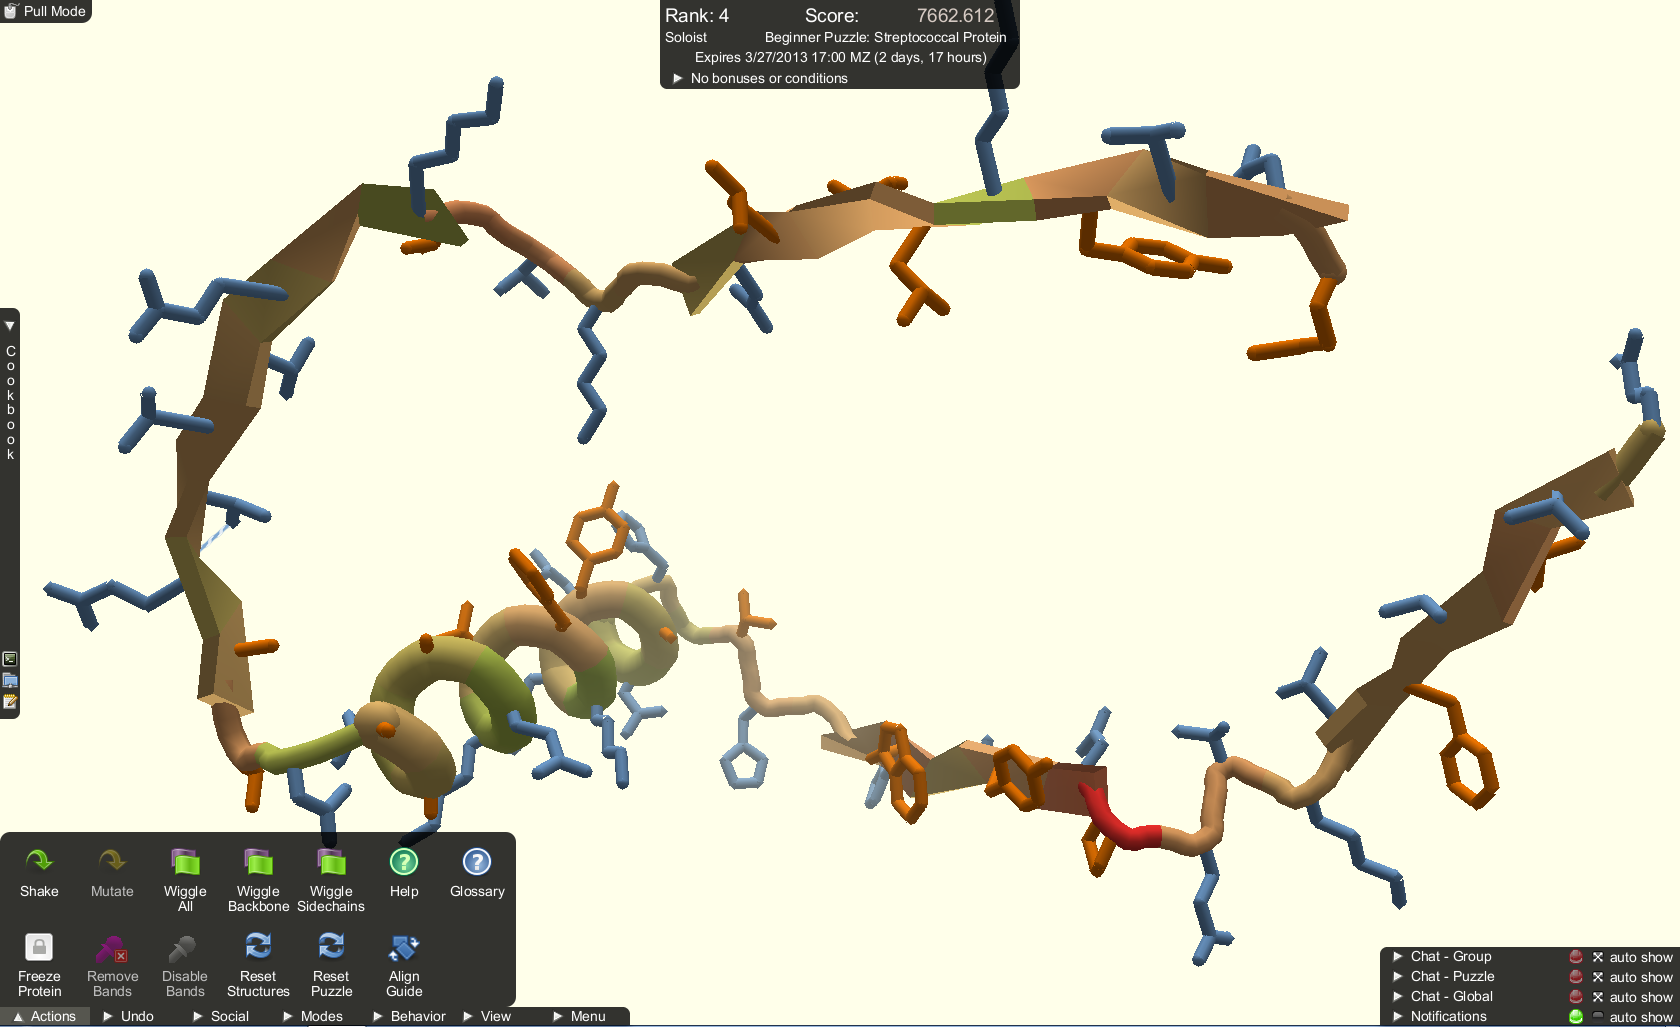
\includegraphics[width=0.8\linewidth]{images/background/foldit-problem.png}
    \caption*{Source: \cite{foldit-protein-problem}}
    \label{fig:foldit-problem}
\end{figure}

Foldit, designed by researchers at the University of Washington, is a game in which gamers solve protein folding patterns, a central challenge in biochemistry, by virtually wiggling, shaking and pulling shapes to create small stable structures, as well as developing their own algorithms for solving protein folding \cite{bourzac2008enlisting}. 

\begin{figure}[ht]
    \centering
    \caption{Foldit - Folded up Streptococcal Protein Puzzle}
    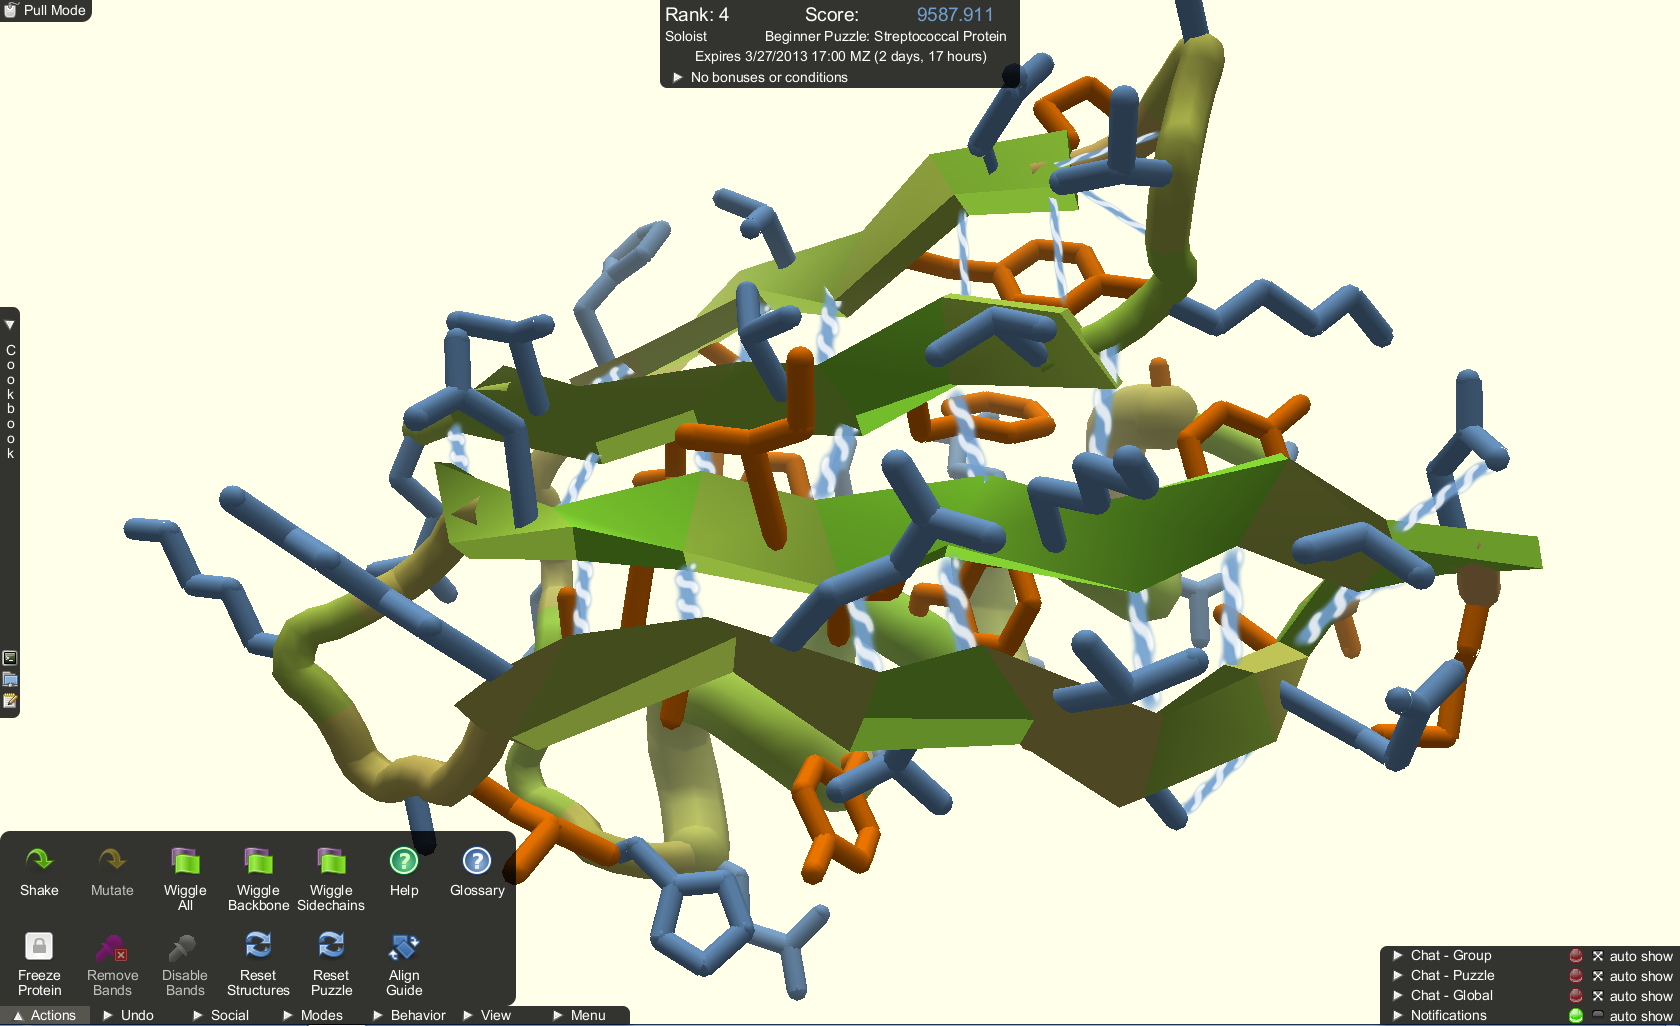
\includegraphics[width=0.8\linewidth]{images/background/foldit-solution.png}
    \caption*{Source: \cite{foldit-protein-solution}}
    \label{fig:foldit-solution}
\end{figure}

As the moment of this article, Foldit has had 20 peer-reviewed articles in a number of journals and conferences \cite{foldit2021publications}. Some relevant breakthroughs are a potential target for HIV drug development \cite{khatib2011crystal}, redesign of the catalyst for the Diels-Alder reaction \cite{eiben2012increased}, and improvement of cryo-electron microscopy atomic model building and refinement \cite{khatib2019building}.

\subsubsection{Gamification in Foldit}

To appeal to the general public, Foldit applies gamification in many different elements. The main objective of the game is to obtain the most stable and folded protein. To encourage this optimization, the user interface assigns a score to the protein, relative to how well it is folded. The best solutions to these puzzles are displayed in a ranking system, to promote competition between users. Another element to aid engagement is social gamification. Users create and join groups, and members of groups can share puzzle solutions. These groups have been found to be useful in training new players.

\subsection{EyeWire}

\begin{figure}[ht]
    \centering
    \caption{EyeWire game interface}
    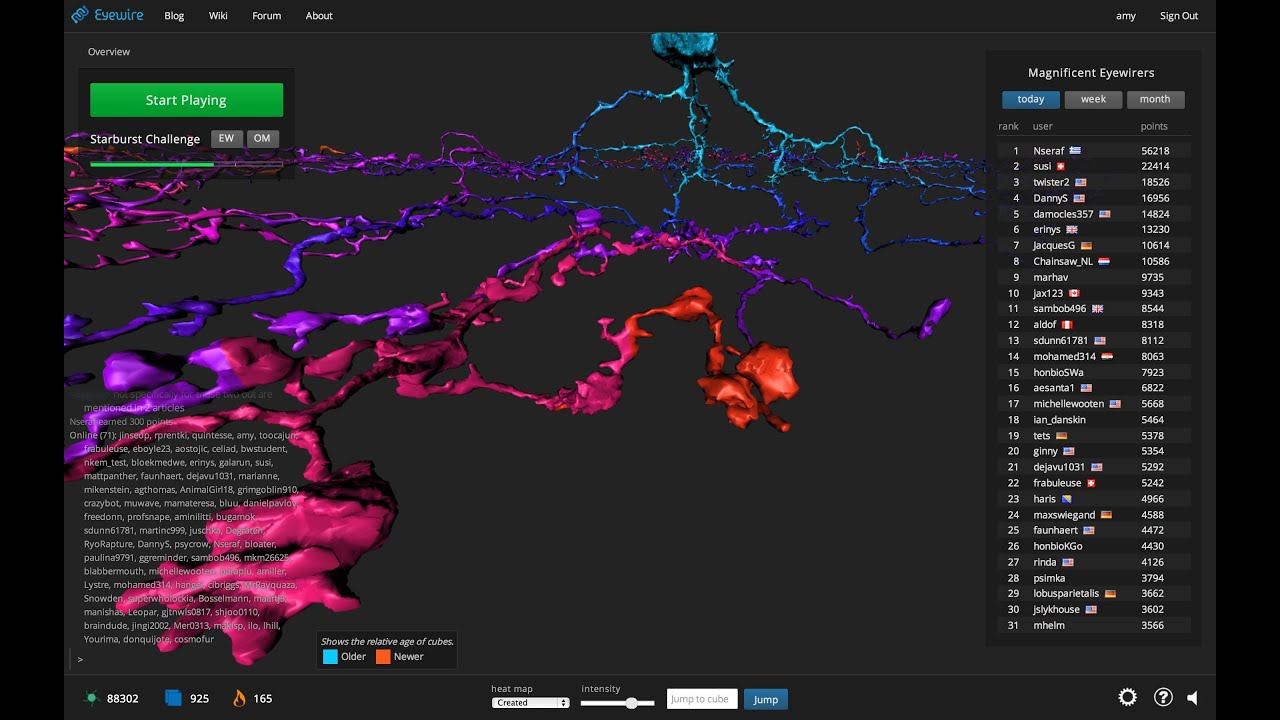
\includegraphics[width=0.8\linewidth]{images/background/eyewire.jpg}
    \caption*{Source: \cite{eyewire2014how}}
    \label{fig:eyewire-game-interface}
\end{figure}

EyeWire is a Web-based citizen science game that aims to create a detailed atlas of the human brain. Nonprofessionals are asked to map connections of neurons which reside in the back of the human eye. This mapping is done through 3D-transformed functional magnetic resonance images (fMRI), and combines crowd contributions with machine learning algorithms to help neuroscientists to achieve a better understanding of visual stimuli processing by humans.

\subsubsection{Gamification in EyeWire}

EyeWire transforms the complex task of brain mapping into smaller (micro) tasks via a gaming interface with several elements associated \cite{seaborn2015gamification}. This has been identified as a positive motivation for a player's participation \cite{tinati2016because}. Other elements such as music, sound effects, interactive tutorials, leaderboard, and a chat interface add to the overall experience, creating a fun experience - according to a survey on EyeWire motivation \cite{tinati2016because}, out of 349 respondents, 57\% considered the the game entertaining.

\subsection{Zooniverse}

\begin{figure}[ht]
    \centering
    \caption{Zooniverse Platform, connecting volunteers with scientists}
    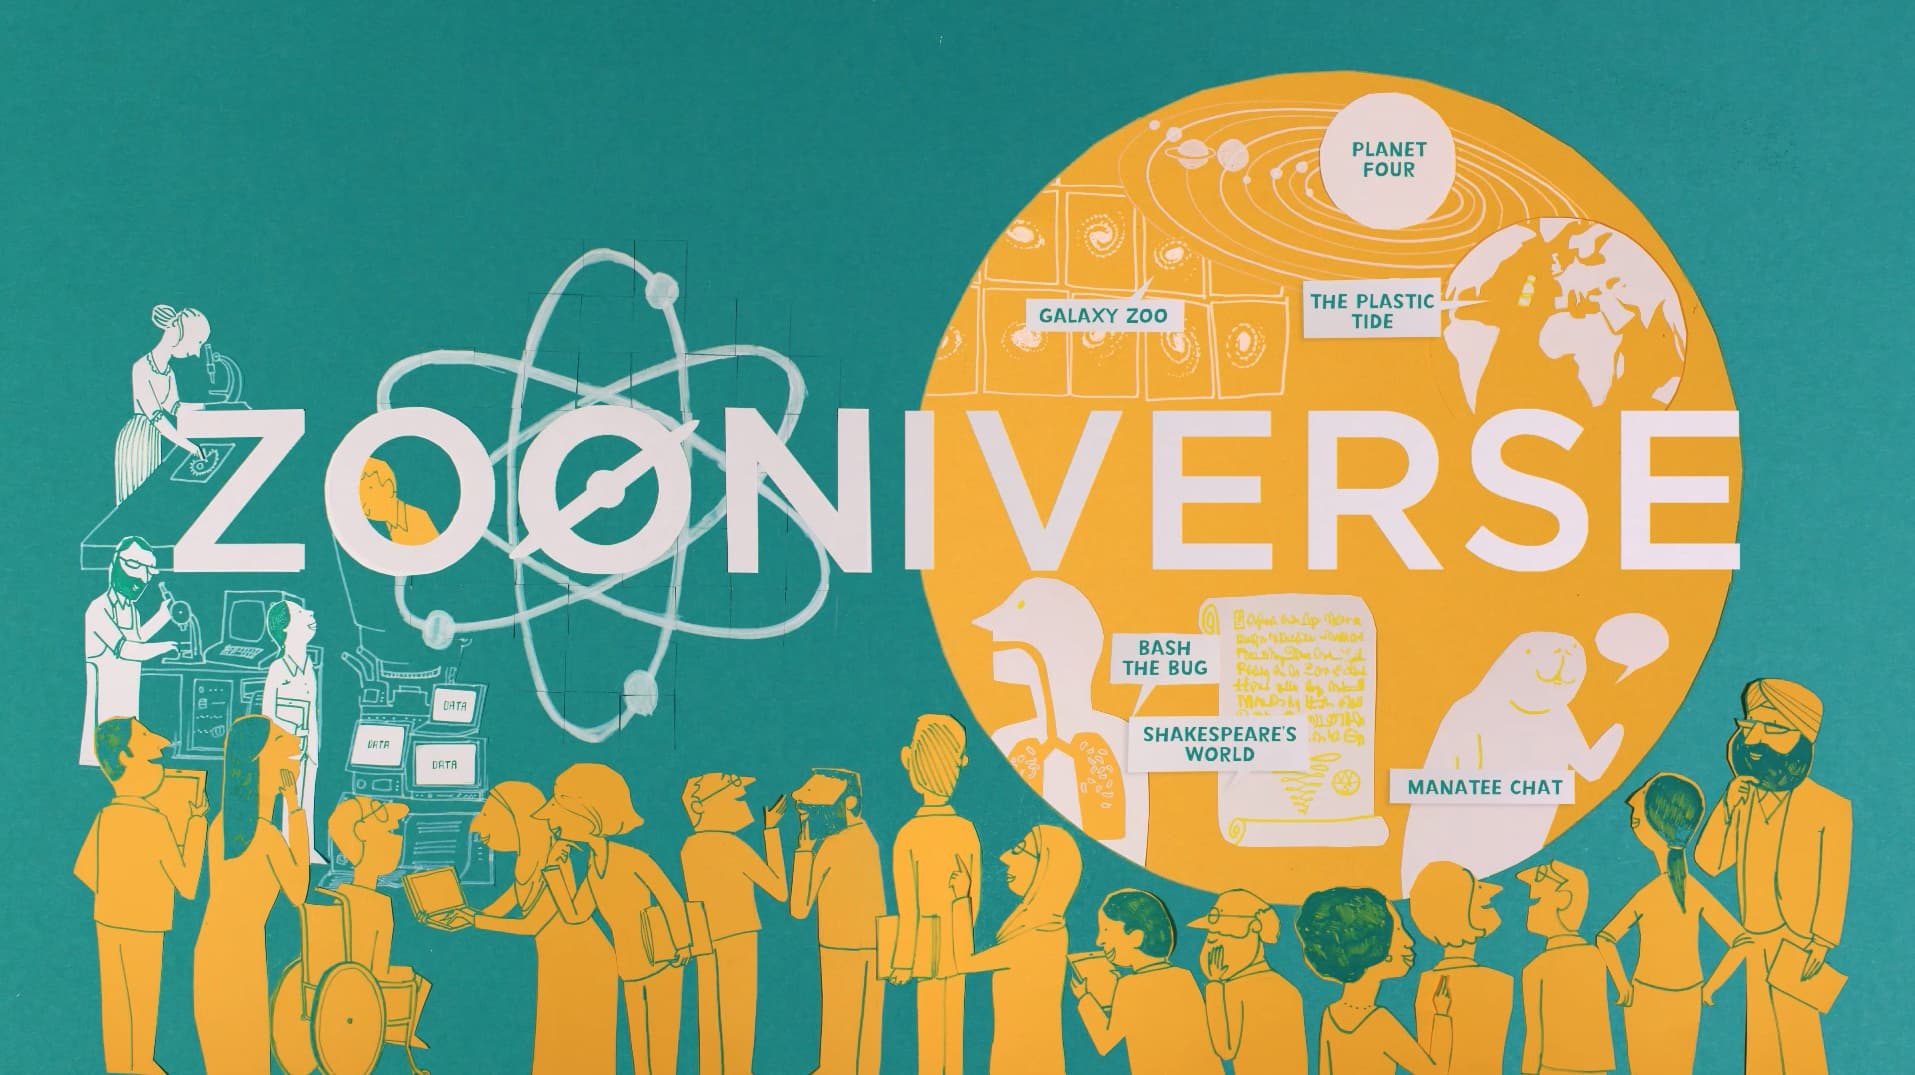
\includegraphics[width=0.7\linewidth]{images/background/zooniverse.jpg}
    \caption*{Source: \cite{zooniverse-logo}}
    \label{fig:foldit-solution}
\end{figure}

Zooniverse is a platform for citizen science projects. It connects more than a million volunteers around the world to assist professional researchers. The platform has a simple interface for input and classification of data, as well as the creation and management of projects.

This collaborative platform has enabled over 300 of scientific publications, with publications on the discovery and classification of stars, planets, supernovas; humanities, animal identification, classification of whale calls, datasets, etc.

\subsection{Galaxy Zoo}

\begin{figure}[ht]
    \centering
    \caption{Hubble's Galaxy Classification Schema to help new players classify galaxies}
    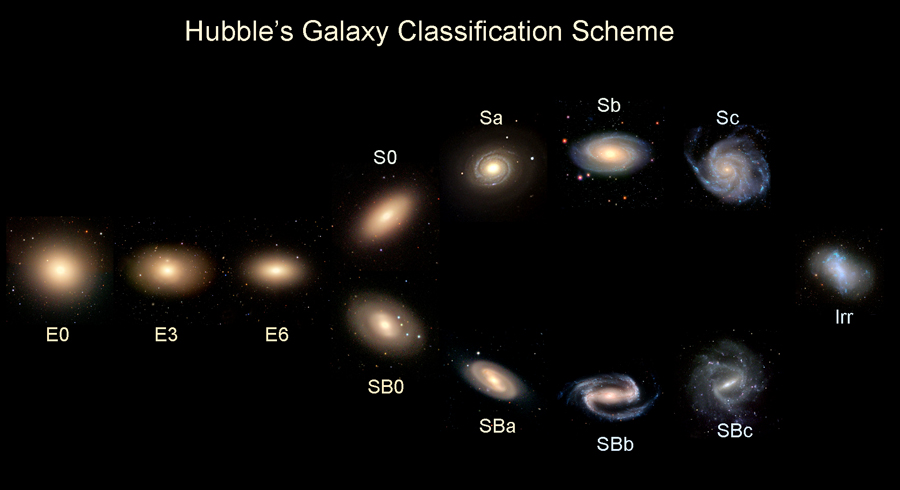
\includegraphics[width=0.8\linewidth]{images/background/galaxyzoo-training.jpg}
    \caption*{Source: \cite{galaxyzoo2010hubble}}
    \label{fig:galaxyzoo-hubble}
\end{figure}

Part of the Zooniverse platform, GalaxyZoo 
https://www.zooniverse.org/projects/zookeeper/galaxy-zoo

\subsubsection{Gamification in Galaxy Zoo}

\subsection{Penguin Watch}

\begin{figure}[ht]
    \centering
    \caption{Penguin Watch interface - Penguins are marked as adults and chicks}
    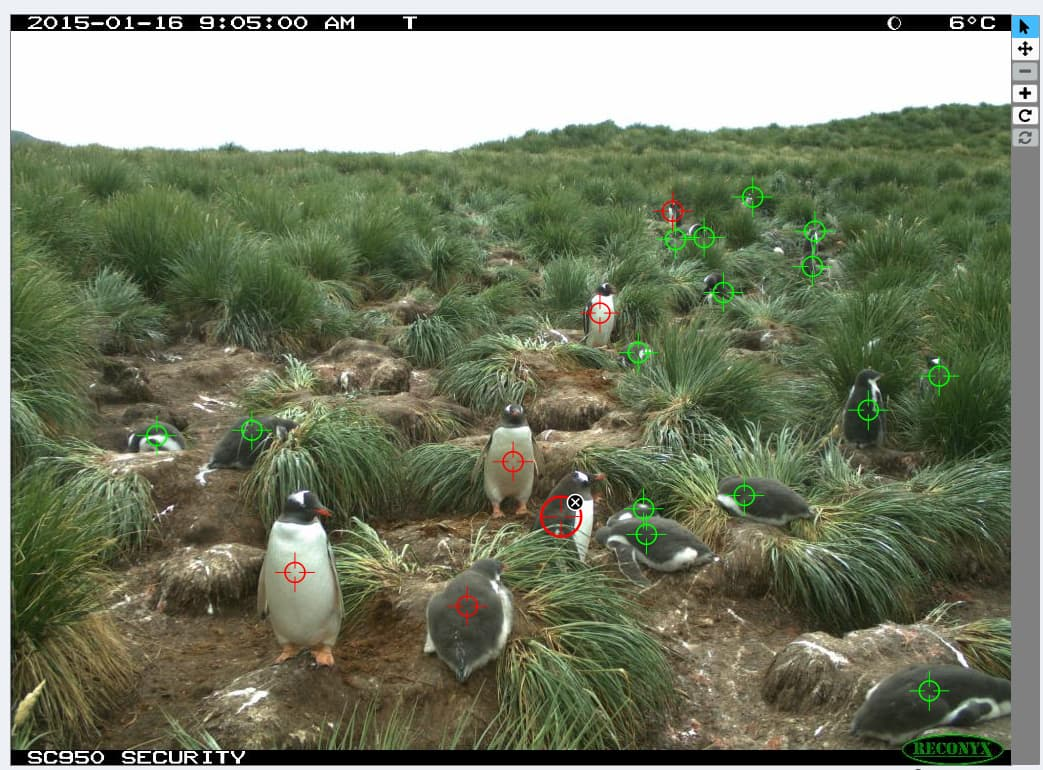
\includegraphics[width=0.8\linewidth]{images/background/penguinwatch.jpg}
    \caption*{Source: \cite{penguin2015watch}}
    \label{fig:oldweather-logbook}
\end{figure}

The Penguin Watch citizen science project states that by monitoring the population change in seabirds like penguins, it is possible to identify changes occurring in the wider ecosystem. These changes can help create health indicators of the marine environment, but the lack of the ability to collect and analyze such amounts of data made a team of researchers create the Penguin Watch initiative. Contributors help identify penguins in images of various sites over the world by using a web interface in Zooniverse.

\subsubsection{Gamification in Penguin Watch}

Like with GalaxyZoo, Penguin Watch runs their contribution platform over Zooniverse. On one hand, Zooniverse is responsible for the infrastructure and service management, while the team at Penguin Watch only analyzes the data. However, since Zooniverse platform has limitations, the use of gamification is limited to social interaction of players.

\subsection{Contributions}

The table \ref{tab:cs-contributions} contains an aggregated list of contributors and contributions from the projects described above.

\begin{table}[h]
    \centering
    \caption{Contribution for online citizen science projects}
    \begin{tabular}{|c|c|c|}
        \hline Project & Contributors & Publications \\
        \hline Foldit & 855,350 \cite{foldit2021players} & 20 \cite{foldit2021publications} \\ 
        \hline EyeWire & 300,000 \cite{eyewire2017players} & 3 \cite{eyewire2021publications} \\ 
        \hline Penguin Watch & 28,500 \cite{penguin2021players} & 10 \cite{penguin2021publications} \\ 
        \hline Galaxy Zoo & 61,149 \cite{galaxyzoo2021players} & 64 \cite{galaxyzoo2021publications} \\ 
        \hline 
    \end{tabular}
    \caption*{Source: Author}
    \label{tab:cs-contributions}
\end{table}

\section{Natural Language Processing}

\subsection{Speech Recognition}

\section{Speech Corpus}

\section{Noisy data}

A common issue with these croudsourced online datasets lies in data quality. Disparities in recorded noise, environment change, recording length variation, and general quality of the recording are intrinsically associated with these contributions, since volunteers have each their own devices and recording conditions. To mitigate these issues, work has been made in the post-processing of these recordings \cite{krishna2019speech}.

\section{Licencing}
\subsection{GPL}
\subsection{CC0}

\section{Systematic Literature Review}

